\documentclass[11pt,letter]{article}
\usepackage{amsmath, amsthm, amssymb}
\usepackage{eucal, mathrsfs, yfonts}
\usepackage{amsfonts}
\usepackage{amssymb}
\usepackage{amsmath}
\usepackage{amsthm}
\usepackage{verbatim}
\usepackage{fancyhdr}
\usepackage{geometry}
\usepackage{setspace}
\usepackage{Tabbing}
\usepackage{lastpage}
\usepackage{extramarks}
\usepackage{chngpage}
\usepackage{soul,color}
\usepackage{graphicx,float,wrapfig}
\usepackage[urlcolor=blue]{hyperref}
\hypersetup{colorlinks=true}

\graphicspath{{./Pictures/}}

%code preamble
\usepackage{color}
\usepackage{xcolor}
\usepackage{listings}

\usepackage{caption}
\DeclareCaptionFont{white}{\color{white}}
\DeclareCaptionFormat{listing}{\colorbox{gray}{\parbox{\textwidth}{#1#2#3}}}
\captionsetup[lstlisting]{format=listing,labelfont=white,textfont=white}

\lstset{language=C++,
               basicstyle=\ttfamily\small,
               keywordstyle=\color{blue}\ttfamily,
               otherkeywords={WIDTH},
               keywords=[2]{__shared__},
               keywordstyle=[2]\color{orange}\ttfamily,
               stringstyle=\color{green}\ttfamily,
               commentstyle=\color{red}\ttfamily,
               breaklines=true,
}
%end code preamble

\topmargin=-0.45in      %
\evensidemargin=0in     %
\oddsidemargin=0in      %
\textwidth=6.5in        %
\textheight=9.0in       %
\headsep=0.25in         %


\newcommand{\HRule}{\rule{\linewidth}{0.5mm}}

\pagestyle{fancy}

%-------------------------------------------------------------------------
%TITLE AND HEADERS
%-------------------------------------------------------------------------

\lhead{Asssignment 4}
\chead{UCID: 22365174}
\rhead{Arturo Pacifico Griffini}

\title{Assignment 4}
\author{Arturo Pacifico Griffini\\
  UCID: 22365174}
\date{}

\begin{document}
%\maketitle
%\input{./title.tex}

\pagebreak

%-------------------------------------------------------------------------
%PROBLEMS
%-------------------------------------------------------------------------


\section{Understanding Vector Increment}

\begin{lstlisting}[label=some-code,caption=incr.cpp ]
#include <cstring>
#include <cstdio>
#include <cstdlib>
#include <string>

#include "clhelp.h"

int main(int argc, char *argv[])
{
  std::string incr_kernel_str;

  /* Provide names of the OpenCL kernels
   * and cl file that they're kept in */
  std::string incr_name_str =
    std::string("incr");
  std::string incr_kernel_file =
    std::string("incr.cl");

  cl_vars_t cv;
  cl_kernel incr;

  /* Read OpenCL file into STL string */
  readFile(incr_kernel_file,
	   incr_kernel_str);

  /* Initialize the OpenCL runtime
   * Source in clhelp.cpp */
  initialize_ocl(cv);

  /* Compile all OpenCL kernels */
  compile_ocl_program(incr, cv, incr_kernel_str.c_str(),
		      incr_name_str.c_str());

  /* Arrays on the host (CPU) */
  float *h_Y, *h_YY;
  /* Arrays on the device (GPU) */
  cl_mem g_Y;

  int n = (1<<20);
  h_Y = new float[n];
  h_YY = new float[n];

  for(int i = 0; i < n; i++)
    {
      h_YY[i] = h_Y[i] = (float)drand48();
    }

  cl_int err = CL_SUCCESS;
  /* CS194: Allocate memory for arrays on
   * the GPU */
  /* Creates a buffer in the cv.context context, with read and write access
   * at the global host adress g_Y, of size sizeof(float)*n. */
  g_Y = clCreateBuffer(cv.context,CL_MEM_READ_WRITE,sizeof(float)*n,NULL,&err);
  CHK_ERR(err);

  /* enqueue commands to write to the buffer g_Y from hos memory.
   * Commands will be queued in cv.commands.
   * true indicates that the write is put on the commands queue.
   * 0 is the offset in bytes in the buffer object to write to.
   * sizeof(float)*n is the size in byte of data being wirtten.
   * h_Y is the address in host memory of the data being written from.
   */
   err = clEnqueueWriteBuffer(cv.commands, g_Y, true, 0, sizeof(float)*n,
			     h_Y, 0, NULL, NULL);
   /* checks whether the write buffer command was succesful. */
  CHK_ERR(err);

  /* declaring the global size of th y dimension to be n. */
  size_t global_work_size[1] = {n};
  /* declaring the size of work groups to be 128 work items. */
  size_t local_work_size[1] = {128};

  /* Sets specific arguments for the kernel incr.
   * 0 is the argument index, sizeof(cl_mem) is the size
   * of the argument, which is the pointer to g_Y.*/
  err = clSetKernelArg(incr, 0, sizeof(cl_mem), &g_Y);
  CHK_ERR(err);

  /* Sets specific arguments for the kernel incr.
   * 1 is the argument index, sizeof(int) is the size
   * of the argument, which is the pointer to n.*/
  err = clSetKernelArg(incr, 1, sizeof(int), &n);
  CHK_ERR(err);

  /* Enqueues a command on cv.commands to execute the
   * kernel incr.cl on the device. Uses linear dimension
   * to specify work groups and items and specifies to use
   * global_work_size work items for the execution and local_work_size
   * as the size of a work group.  */
  err = clEnqueueNDRangeKernel(cv.commands,
			       incr,
			       1,//work_dim,
			       NULL, //global_work_offset
			       global_work_size, //global_work_size
			       local_work_size, //local_work_size
			       0, //num_events_in_wait_list
			       NULL, //event_wait_list
			       NULL //
			       );
  CHK_ERR(err);

  /* Read result of GPU on host CPU */
  err = clEnqueueReadBuffer(cv.commands, g_Y, true, 0, sizeof(float)*n,
			    h_Y, 0, NULL, NULL);
  CHK_ERR(err);

  /* Check answer */
  bool er = false;
  for(int i = 0; i < n; i++)
    {
      float d = (h_YY[i] + 1.0f);
      if(h_Y[i] != d)
	{
	  printf("error at %d :(\n", i);
	  er = true;
	  break;
	}
    }
  if(!er)
    {
      printf("CPU and GPU results match\n");
    }

  uninitialize_ocl(cv);

  delete [] h_Y;
  delete [] h_YY;

  clReleaseMemObject(g_Y);
  return 0;
}
\end{lstlisting}


\begin{lstlisting}[label=some-code,caption=incr.cl ]
/* The __kernel qualifier declares a function
 * that can be executed by an application running
 * on an OpenCL device.
 * The __global qualifier declares that the pointer
 * to Y can point only to the global memory pool.
 * i.e. Y must be in the global memory pool.*/
__kernel void incr (__global float *Y, int n)
{
  /* get_global_id(0) returns the global index of the
   * of the current work item. The 0 argument indicates
   * dimension 0. You can give dimensional indices to
   * work items. In this case it is linear. */
  int idx = get_global_id(0);
  /* If the global index of the work item is less than
   * the size of the array at Y, add 1 to the value of the
   * at adress Y + idx. */
  if(idx < n)
    {
      Y[idx] = Y[idx] + 1.0f;
    }
}

\end{lstlisting}

\section{Implement Vector Addition}

\begin{lstlisting}[label=some-code,caption=vvadd.cl]
__kernel void vvadd (__global float *Y, __global float *A, __global float *B,
	 int n)
{
  /* CS194: implement the body of this kernel */
  /* Let every work item do an addition. */
  int id = get_global_id(0);
  if (id < n)
     Y[id] = A[id] + B[id];
}
\end{lstlisting}

\begin{lstlisting}[label=some-code,caption=vvadd.cpp]
#include <cstring>
#include <cstdio>
#include <cstdlib>
#include <string>

#include "clhelp.h"

int main(int argc, char *argv[])
{
  std::string vvadd_kernel_str;

  /* Provide names of the OpenCL kernels
   * and cl file that they're kept in */
  std::string vvadd_name_str = 
    std::string("vvadd");
  std::string vvadd_kernel_file = 
    std::string("vvadd.cl");

  cl_vars_t cv; 
  cl_kernel vvadd;

  /* Read OpenCL file into STL string */
  readFile(vvadd_kernel_file,
	   vvadd_kernel_str);
  
  /* Initialize the OpenCL runtime 
   * Source in clhelp.cpp */
  initialize_ocl(cv);
  
  /* Compile all OpenCL kernels */
  compile_ocl_program(vvadd, cv, vvadd_kernel_str.c_str(),
		      vvadd_name_str.c_str());
  
  /* Arrays on the host (CPU) */
  float *h_A, *h_B, *h_Y;
  /* Arrays on the device (GPU) */
  cl_mem g_A, g_B, g_Y;

  /* Allocate arrays on the host
   * and fill with random data */
  int n = (1<<20);
  h_A = new float[n];
  h_B = new float[n];
  h_Y = new float[n];
  bzero(h_Y, sizeof(float)*n);
  
  for(int i = 0; i < n; i++)
    {
      h_A[i] = (float)drand48();
      h_B[i] = (float)drand48();
    }

  /* CS194: Allocate memory for arrays on 
   * the GPU */
  cl_int err = CL_SUCCESS;
  
  /* CS194: Here's something to get you started  */
  g_Y = clCreateBuffer(cv.context,CL_MEM_READ_WRITE,sizeof(float)*n,NULL,&err);
  CHK_ERR(err);
  g_A = clCreateBuffer(cv.context,CL_MEM_READ_WRITE,sizeof(float)*n,NULL,&err);
  CHK_ERR(err);
  g_B = clCreateBuffer(cv.context,CL_MEM_READ_WRITE,sizeof(float)*n,NULL,&err);
  CHK_ERR(err);
  
  /* CS194: Copy data from host CPU to GPU */
  err = clEnqueueWriteBuffer(cv.commands, g_Y, true, 0, sizeof(float)*n, h_Y, 0, NULL, NULL);
  CHK_ERR(err);
  err = clEnqueueWriteBuffer(cv.commands, g_A, true, 0, sizeof(float)*n, h_A, 0, NULL, NULL);
  CHK_ERR(err);
  err = clEnqueueWriteBuffer(cv.commands, g_B, true, 0, sizeof(float)*n, h_B, 0, NULL, NULL);
  CHK_ERR(err);
 
  /* CS194: Define the global and local workgroup sizes */
  size_t global_work_size[1] = {n};
  size_t local_work_size[1] = {128};
  
  /* CS194: Set Kernel Arguments */
  err  = clSetKernelArg(vvadd, 0, sizeof(cl_mem), &g_Y);
  CHK_ERR(err);
  err = clSetKernelArg(vvadd, 1, sizeof(cl_mem), &g_A);
  CHK_ERR(err);
  err = clSetKernelArg(vvadd, 2, sizeof(cl_mem), &g_B);
  CHK_ERR(err);
  err = clSetKernelArg(vvadd, 3, sizeof(int), &n);
  CHK_ERR(err);

  /* CS194: Call kernel on the GPU */
  err = clEnqueueNDRangeKernel(cv.commands,
                               vvadd,
                               1,//work_dim,
                               NULL, //global_work_offset
                               global_work_size, //global_work_size
                               local_work_size, //local_work_size
                               0, //num_events_in_wait_list
                               NULL, //event_wait_list
                               NULL //
                               );
  /* Read result of GPU on host CPU */
  err = clEnqueueReadBuffer(cv.commands, g_Y, true, 0, sizeof(float)*n,
			    h_Y, 0, NULL, NULL);
  CHK_ERR(err);

  /* Check answer */
  for(int i = 0; i < n; i++)
    {
      float d = h_A[i] + h_B[i];
      if(h_Y[i] != d)
    	{
    	  printf("error at %d :(\n", i);
    	  break;
    	}
    }

  /* Shut down the OpenCL runtime */
  uninitialize_ocl(cv);
  
  delete [] h_A; 
  delete [] h_B; 
  delete [] h_Y;
  
  clReleaseMemObject(g_A); 
  clReleaseMemObject(g_B); 
  clReleaseMemObject(g_Y);
  
  return 0;
}
\end{lstlisting}

\section{Implement Matrix Multiply}

\begin{lstlisting}[label=some-code,caption=matmul.cl]
__kernel void matmul(__global float *Y, __global float *A, __global float *B, 
	 int n)
{
  /* CS194: Implement the body of this kernel */
  /* assign each 2d position in the result matrix to each work item. */
  int x = get_global_id(0);
  int y = get_global_id(1);
  float val = 0;
  /* Compute dot product to put the posisiotn (x, y). */
  for (int k = 0; k < n; k++) 
      val += A[y * n + k] * B[k * n + x];
  Y[y * n + x] = val;
}
\end{lstlisting}


\begin{lstlisting}[label=some-code,caption=matmul.cpp]
#include <cstring>
#include <cstdio>
#include <cstdlib>
#include <string>
#include <cassert>
#include <cmath>

#include "clhelp.h"

void sqr_sgemm(float *Y, float *A, float *B, int n);

int main(int argc, char *argv[])
{
  std::string matmul_kernel_str;
 
  std::string matmul_name_str = 
    std::string("matmul");
  std::string matmul_kernel_file = 
    std::string("matmul.cl");

  cl_vars_t cv; 
  cl_kernel matmul;
  
  readFile(matmul_kernel_file,
	   matmul_kernel_str);
  
  initialize_ocl(cv);
  
  compile_ocl_program(matmul, cv, matmul_kernel_str.c_str(),
		      matmul_name_str.c_str());
  
  float *h_A, *h_B, *h_Y, *h_YY;
  cl_mem g_A, g_B, g_Y;
  int n = (1<<10);
  h_A = new float[n*n];
  assert(h_A);
  h_B = new float[n*n];
  assert(h_B);
  h_Y = new float[n*n];
  assert(h_Y);
  h_YY = new float[n*n];
  assert(h_YY);
  bzero(h_Y, sizeof(float)*n*n);
  bzero(h_YY, sizeof(float)*n*n);
  
  for(int i = 0; i < (n*n); i++)
    {
      h_A[i] = (float)drand48();
      h_B[i] = (float)drand48();
    }

  cl_int err = CL_SUCCESS;
  /* CS194: Allocate Buffers on the GPU.
   *...We're already allocating the Y buffer
   * on the GPU for you */
  g_Y = clCreateBuffer(cv.context,CL_MEM_READ_WRITE,
		       sizeof(float)*n*n,NULL,&err);
  CHK_ERR(err);
  g_A = clCreateBuffer(cv.context,CL_MEM_READ_WRITE,
                       sizeof(float)*n*n,NULL,&err);
  CHK_ERR(err);
  g_B = clCreateBuffer(cv.context,CL_MEM_READ_WRITE,
                       sizeof(float)*n*n,NULL,&err);
  CHK_ERR(err);

  /* CS194: Copy data from host CPU to GPU */
  err = clEnqueueWriteBuffer(cv.commands, g_Y, true, 0, sizeof(float)*n*n, h_Y, 0, NULL, NULL);
  CHK_ERR(err);
  err = clEnqueueWriteBuffer(cv.commands, g_A, true, 0, sizeof(float)*n*n, h_A, 0, NULL, NULL);
  CHK_ERR(err);
  err = clEnqueueWriteBuffer(cv.commands, g_B, true, 0, sizeof(float)*n*n, h_B, 0, NULL, NULL);
  CHK_ERR(err);

  /* CS194: Create appropriately sized workgroups */
  size_t global_work_size[2] = {n, n};
  size_t local_work_size[2] = {16, 16};
  
  /* CS194: Set kernel arguments 
   * 0 => result matrix Y, 1 => matrix A, 2 => matrix B
   * 3 => size of matrices.*/
  err = clSetKernelArg(matmul, 0, sizeof(cl_mem), &g_Y);
  CHK_ERR(err);
  err = clSetKernelArg(matmul, 1, sizeof(cl_mem), &g_A);
  CHK_ERR(err);
  err = clSetKernelArg(matmul, 2, sizeof(cl_mem), &g_B);
  CHK_ERR(err);
  err = clSetKernelArg(matmul, 3, sizeof(int), &n);
  CHK_ERR(err);

  double t0 = timestamp();
  /* CS194: Launch matrix multiply kernel
   * Here's a little code to get you started.. 
   err = clEnqueueNDRangeKernel(cv.commands,...
			       );
   CHK_ERR(err);
   err = clFinish(cv.commands);
   CHK_ERR(err);
  */
  /* All as in incr and vvadd but with two working 
   * dimensions this time. */
  err = clEnqueueNDRangeKernel(cv.commands,
                               matmul,
                               2,//work_dim,
                               NULL, //global_work_offset
                               global_work_size, //global_work_size
                               local_work_size, //local_work_size
                               0, //num_events_in_wait_list
                               NULL, //event_wait_list
                               NULL //
                               );
  CHK_ERR(err);
  err = clFinish(cv.commands);
  CHK_ERR(err);
  t0 = timestamp()-t0;

  /* Read result of GPU on host CPU */
  err = clEnqueueReadBuffer(cv.commands, g_Y, true, 0, sizeof(float)*n*n,
			    h_Y, 0, NULL, NULL);
  CHK_ERR(err);
  err = clFinish(cv.commands);
  CHK_ERR(err);

  double t1 = timestamp();
  sqr_sgemm(h_YY, h_A, h_B, n);
  t1 = timestamp()-t1;

  for(int i = 0; i < (n*n); i++)
    {
      double d = h_YY[i] - h_Y[i];
      d *= d;
      if(d > 0.0001)
	{
	  printf("CPU and GPU results do not match!\n");
	  break;
	}
    }
  uninitialize_ocl(cv);
  
  delete [] h_A; 
  delete [] h_B; 
  delete [] h_Y;
  delete [] h_YY;

  clReleaseMemObject(g_A); 
  clReleaseMemObject(g_B); 
  clReleaseMemObject(g_Y);
  
  double gpu_flops_s = (2.0 * pow((double)n, 3.0)) / t0;
  printf("GPU: %g gflops/sec\n", gpu_flops_s / (1e9));

  double cpu_flops_s = (2.0 * pow((double)n, 3.0)) / t1;
  printf("CPU: %g gflops/sec\n", cpu_flops_s / (1e9));
  return 0;
}
\end{lstlisting}

%\begin{figure}[h]
%\centering
%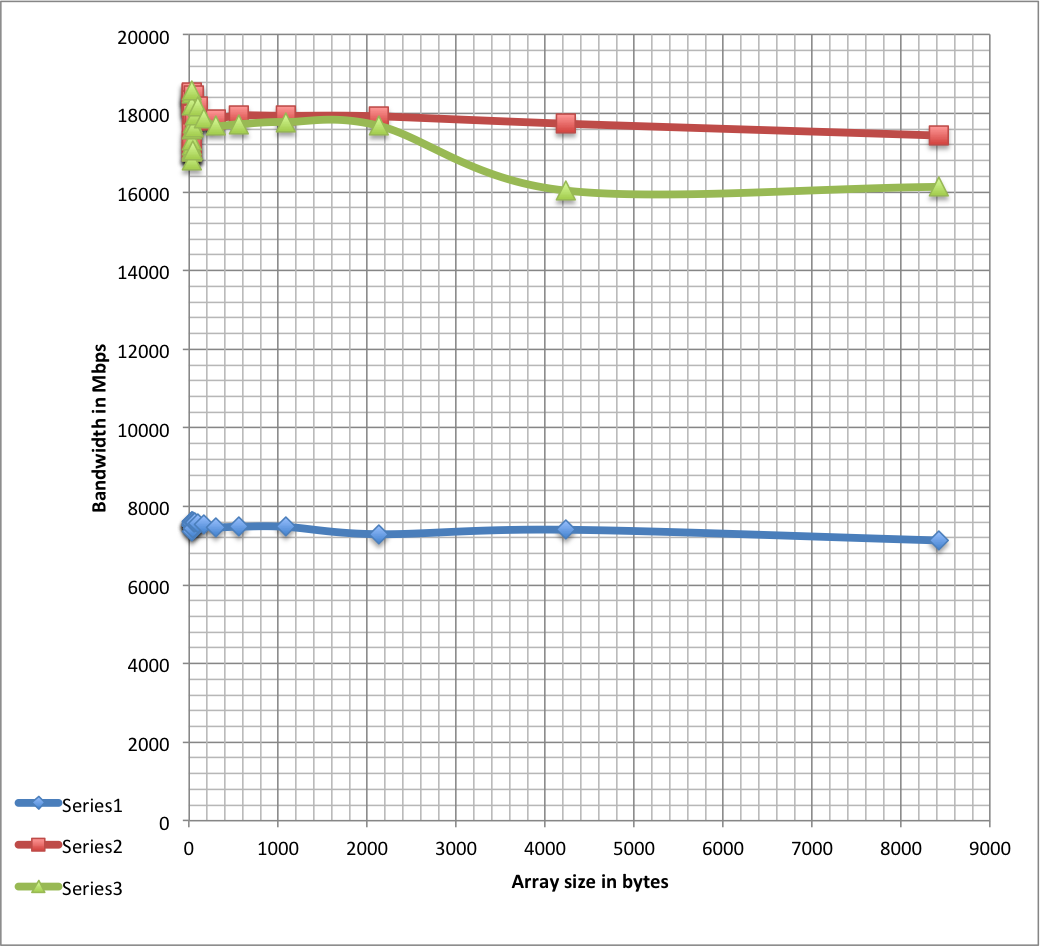
\includegraphics[width=0.8\textwidth]{graph_mem.png}
%\caption{series 1: inefficient routine; series 2: simd\_memcpy; series 3: simd\_memcpy\_cache}
%\label{fig:awesome_image}
%\end{figure}



\end{document}








% \begin{lstlisting}[label=some-code,caption=Some Code]
% public void here() {
% goes().the().code()
% }
% \end{lstlisting}








